\chapter{Implementácia}
Implementáciu celého systému sme rozdelili na 3 časti. Servrová časť obsahuje zdrojové kódy v pythone pre backend a producentov úloh pre celery. Klientska čast zapuzdruje užívateľské rozhranie v Angular 2 a nástroje potrebné na vývoj a preklad zdrojových kódov. V deployment časti sú skripty ktoré plne automatizujú nasadenie aplikácie na linuxový server.


\section{Servrová časť}
Hlavnou funkcionalitou tejto časti je obslúžiť požiadavky prichádzajúce ako http volania, spracovať ich a vrátiť výsledok do formáte JSON. Backend sa teda priamo nestará o obslúženie užívateľských akcií, ani o routovanie a len odpovedá na volania z klienta. V REST api vystavujeme tieto metódy:

 \begin{minipage}{0.9\linewidth}
 	\centering
 	\missingfigure[figheight=10cm]{tabulka rest api}
 	%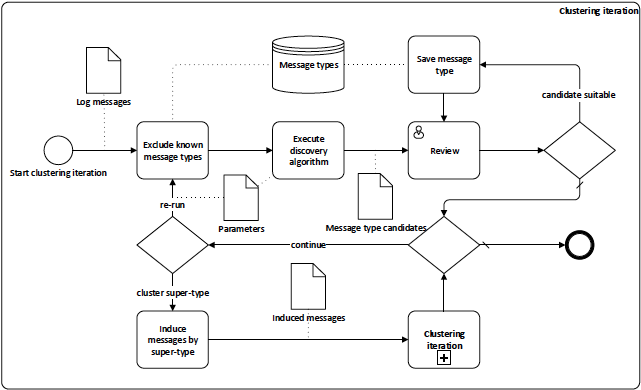
\includegraphics[width=\textwidth]{images/RURC.png} 	
 \end{minipage}
 
 
Pri implementácií sme sa intenzívne spoliehali framework Django. Django obsahuje veľké množstvo modulov, z ktorých sme v našej práci síce využili len malú podmnožinu, ale zásadne nám zjednodušila celú implementáciu. Funkcionalita je rozdelená do samostatných súborov alebo modulov pre jednoduchý a prehľadný kód

\subsection*{Django ORM}
Pre prístup k dátam z databázy je v celej aplikácii použité objektovo relačné mapovanie zakomponované priamo v Djangu. Využitie Django ORM vo väčšine prípadov vývojára úplne odprostí od potreby implementovať DAL - vrstvu pre prístup k dátam, ako je zvyklé napr. Java alebo .NET. Django ORM používa potomkov triedy \emph{django.db.models.Model}, ďalej nazývaných ako modely, na zadefinovanie štruktúry dát a pôsobí ako jediný prístupový k dátam. Každý model reprezentuje tabuľku v databáze a jeho objekt tohto typu jeden riadok v databáze. 

\begin{figure}[htbp]
\centering
\begin{minipage}{0.9\textwidth}
\lstset{tabsize=4,columns=flexible,breaklines=true,breakatwhitespace=true, showstringspaces=false}
\begin{lstlisting}
class Source(models.Model):
    source = models.CharField(max_length=255, blank=False, db_index=True)
    version = models.CharField(max_length=50)

    class Meta:
        unique_together = ('source', 'version')
\end{lstlisting} 		
\end{minipage} 
\caption{Databázovy model typu Source}
\label{fig:static-analysis}
\end{figure}

\subsection*{Django migrations}
Na vytvorenie databázového schématu používame Django migrations. Použitím Django migrations vývojári nemusia písať ddl scripty a modelujú schéma vytváraním tried v jazyku python. Prvotné schéma je vygenerované automaticky, každá ďalšia zmena kódu spôsobí vygenerovanie novej migrácie, ktorá je následne aplikovaná na databázové tabuľky. Tento spôsob sa ukázal ako veľmi nápomocný v deployment scriptoch, kde jednoducho spustíme migráciu príkazom \emph{python manage.py migrate} a nepotrebujeme dodatočného sql klienta na vytvorenie schématu. Zároveň týmto spôsobom vieme do aplikácie aj vložiť iniciálne data.

\subsection{Implementácia Extended Nagappan-Vouk}
Implementácia sa snaží byť čo najrýchlejšia, preto používame knižnicu \emph{multiprocessing}. Väčšina vykonávaných metód najprv rozdelí problém na menšie časti, spočíta výsledok podproblému v novom procese a následne problém spojí. 
\par  Začína predspracovaní, v ktorom pre každú správu hľadáme sekvenčným prechodom cez už uložené parsovacie vzory ten správny. Ak existuje daná správa je z ďalšieho spracovania vylúčená. Uznávame, že táto operácia nie je veľmi efektívna ako už bolo zmienené v \ref{sec:data-mining} a s narastajúcim počtom uložených správ značne zhorší celkový čas spracovania, preto implementácia tejto operácie môže byť v budúcnosti  jednoducho zameniteľná za riešenie založené na REtrie. Nasleduje samotný beh algoritmu, ktorého výsledky sú uložené do Redisu. Ako návratova hodnota je použitý objekt ktorý obsahuje štatistiku vytvorenú z týchto výsledkov a textovú reprezentáciu parsovacích vzorov.

\begin{figure}[htbp]
 \centering 
 \begin{minipage}{0.95\linewidth}
 	\centering
 	\missingfigure[figheight=10cm]{diagram komponent}
 	%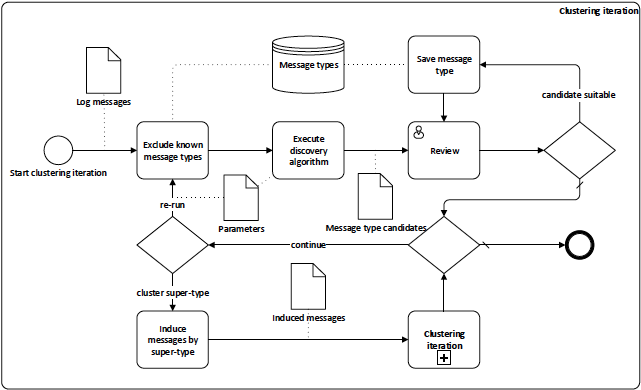
\includegraphics[width=\textwidth]{images/RURC.png} 	
 \end{minipage}
  \caption{ERD diagram vzorov}
  \label{fig:erd-patterns}
\end{figure}

\subsection{Prevod medzi formátmi parsovacích vzorov}
\label{sec:format-transformation}

Pri prevode medzi týmito formátmi potrebujeme mať vopred známu sadu typov regulárnych výrazov, voči ktorým budeme konverziu prevádzať. Je žiadúce aby táto sada nebola konštantná pre všetky parsovacie vzory, ale aby bolo možné ju zadať pre vybrané parsovacie vzory. Z tohto dôvodu nie je transformácia medzi formátmi prevádzaná pri uložení parsovacie vzoru, ale je vykonaná on demand pre zadanú sadu typov algoritmom \ref{fig:pattern-transformation}

\begin{figure}[htbp]
\centering
\begin{minipage}{0.9\textwidth}
\lstset{tabsize=4,columns=flexible,breaklines=true,breakatwhitespace=true, showstringspaces=false}
\begin{lstlisting}
def transform_pattern_to_regex(pattern, pattern_lines, regex_types):
    types_tab = build_pattern_types_tab(pattern, pattern_lines, regex_types)

    transformed_patterns = {}
    pattern_idx = 0
    for line_key, types in types_tab.items():

        idx = 0
        replacements = []
        replacement = ''
        for words_in_groups in line_key.split():
            replacement = ''
            for words_in_group in words_in_groups:
                replacement.append('%{{{name}:var{idx}}}'.format(name=types[idx], idx=idx))
                idx += idx
            replacements.append(replacement)
            
        transformed_patterns['pattern' + pattern_idx] = replace_groups_text(pattern, replacements)

    return transformed_patterns


def build_pattern_types_tab(pattern, pattern_lines, regex_types):
    pattern_types = {}

    for line in pattern_lines:
        pattern_match = pattern.match(line)
        types = []
        keys = []
        pattern_groups = pattern_match.groups()
        for pattern_group in pattern_groups:
            words = pattern_group.split()
            for word in words:
                types.append(find_first_suitable_regex_type(word, regex_types))
            keys.append(str(len(words)))
        line_key = ','.join(keys)
        update_types(pattern_types, line_key, types)

    return pattern_types
\end{lstlisting} 		
\end{minipage} 
\caption{Databázovy model typu Source}
\label{fig:pattern-transformation}
\end{figure}

Hlavný rozdiel medzi popisovanými formátmi je ten, že pokým nativný formát algoritmu Extended Naggap-Vouk skracuje výskyt viacerých parametrov v rade, REtrie formát tento zápis nepozná. Preto vo výsledku z jedného parsovacieho vzoru, môže vzniknúť až 

\begin{align*}
\prod_{group \in groups} group.upper\_bound - group.lower\_bound
\end{align*}

nových vzorov. Ďalší rozdiel je neprítomnosť typu parametra v pôvdnom formáte.


\section{Klientská časť}


\subsection{Angular 2}
Angular 2 je relativne nový komponentovo orientovaný javascriptový framework, ktorý odstraňuje nedostatky pôvodnej verzie. Aplikácie sa v Angulare 2 píšu buď v Typescripte alebo vo verziách ECMAScript 5 resp. 6. Ani jedna varianta zatiaľ nie je plne podporovaná dnešnými prehliadačmi, preto je nutná transkompilácia. My sme použili Typescript, nadstavbu javascriptu, ktorý zavádza statické typovanie a prvky objektovo orientovaného programovania ako typy, triedy, moduly a pod. čo považujeme za veľkú výhodu. Základné stavebné prvky sú

\begin{enumerate}
 \item Modul, zapuzdruje funkcionalitu ktorá vykonáva jednu úlohu. Funguje podobne ako OSGi modul, kde modul vidí len komponenty definované v samotnom module a komponenty ktoré modul explicitne importuje. Zároveň modul špecifikuje, ktoré komponenty budú viditeľné zvonka balíčka.
 \item Komponenta, základny prvok aplikácie. Definuje aplikačnú logiku a interaguje so šablónou cez rozhranie vlastností a metód. Potrebná komfigurácia komponenty je zabezpečená cez metadáta
 \item Šablóna, html stránka obohatená o značky z jazyka Angular. Definuje ako bude zobrazená komponenta. Zároveň obsahuje značkovanie pre prepojenie dát, ktoré určuje ako sú vymieňané data medzi komponentov a šablónov. V predošlej verzii Angularu sa vždy jednalo o obojsmerné prepojenie, čo spôsobovalo výkonnostné problémy. Vo verzii 2 si vieme toto prepojenie zašpecifikovať a vyhnúť sa tak týmto problémom.
 \item Servisná služba, je to trieda, ktorá obsahuje funkcie na vykonanie špecifických úloh potrebných aplikáciou. 
 \item Dependency injection je spôsob založený na rovnomenno návrhovom vzore ktorým Angular poskytuje servisným službám a komponentám závislosti.
\end{enumerate}

\subsubsection*{Podporné nástroje}
Aplikácie písané v Angulare 2 sú závislé na knižniciach tretích strán ako aj na knižniciach samotného Angularu. Na správu týchto závislostí používame všeobecne polulárny Node.js a jeho balíčkovací systém npm. Na správu kódu samotného používame Webpack, jednoduchý baličkovač zdrojových kódov. Webpack ponúka široké možnosti ako zdrojové kódy upraviť pred výsledým zabalením do archívu a zároveň možnosť vystaviť tieto kódy v rámci vývojového servra, čo sme pri vývoji vo veľkej miere využívali. V našom systéme Webpack pred výsledným zabalením zdrojové kódy minimalizuje a prevedie optimalizácie. Oba tieto nástroje sme ovládali a nastavovali cez nástroj Angular CLI, ktorý umožnuje vygenerovať si projekt už obsahujúci najčastejšiu konfiguráciu. 

\subsection{Menu aplikácie}
Menu aplikácie obsahuje 3 položky. Prvá polož Miner obsahuje komponentu, ktorá slúži na samotné odhaľovanie parsovacích vzorov.


\subsection{Miner}
Na začiatku je možné určiť aplikáciu z ktorej analyzované správy pochádzajú a jej verziu. Ďalej môžme určiť či chceme analyzovať správy z  logovacieho súboru ktorý nahrajeme alebo použijeme správy, ktoré už sú v systéme nahrané a neboli zatiaľ finálne analyzované.

\begin{figure}[htbp]
 \centering 
 \begin{minipage}{0.95\linewidth}
 	\centering
 	\missingfigure[figheight=5cm]{Menu aplikacie}
 	%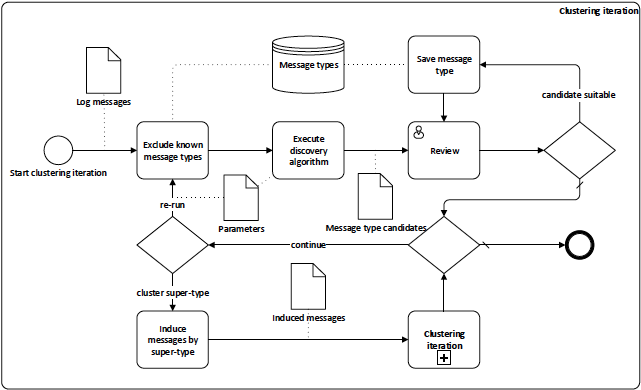
\includegraphics[width=\textwidth]{images/RURC.png} 	
 \end{minipage}
  \caption{Trvanie eng.py }
  \label{fig:eng-duration}
\end{figure}

Po tomto kroku máme pred sebou rozhranie, ktorým budeme upravovať a spúšťať analýzu. Po upresnení oddeľovačov a q-percentilu užívateľ spustí analýzu. Po obdržaní výsledkov je užívateľovi prezentovaná tabuľka, ktorej hlavnú časť tvoria navrhované parsovacie vzory. V tabuľke napravo je tlačidlo, ktorým užívateľ daný parsovací vzor potvrdí ako finálny. Pre potreby spresňujúcej analýzy je pri každom vzore vľavo checkbox. Pri označení ľubovoľného počtu navrhovaných vzorov a následnej analýze sú ako vstupné správy brané len tie, ktoré prislúchali k označeným vzorom. Výsledky spresňujúcej analýzy sú vložené do tabuľky tak, že novo navrhované parsovacie vzory sú pripojené ako potomkovia vzoru z ktorého vznikli a vytvárajú tak stromovú štruktúru. Tento proces vieme opakovať až kým nefinalizujeme všetky parsovacie vzory alebo sa možme rozhodnúť začat novú analýzu.

\begin{figure}[htbp]
 \centering 
 \begin{minipage}{0.95\linewidth}
 	\centering
 	\missingfigure[figheight=5cm]{Zadavanie source}
 	%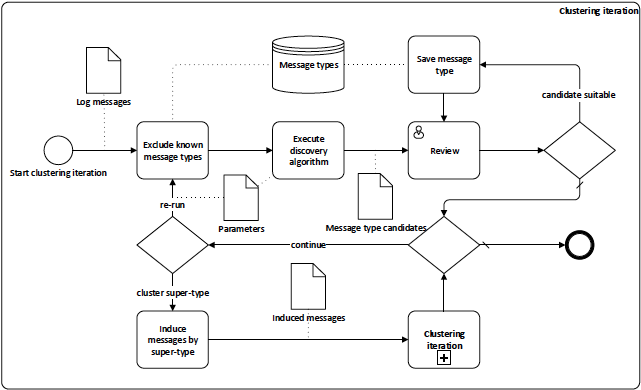
\includegraphics[width=\textwidth]{images/RURC.png} 	
 \end{minipage}
  \caption{Trvanie eng.py }
  \label{fig:eng-duration}
\end{figure}

\begin{figure}[htbp]
 \centering 
 \begin{minipage}{0.95\linewidth}
 	\centering
 	\missingfigure[figheight=5cm]{Proces analyzy}
 	%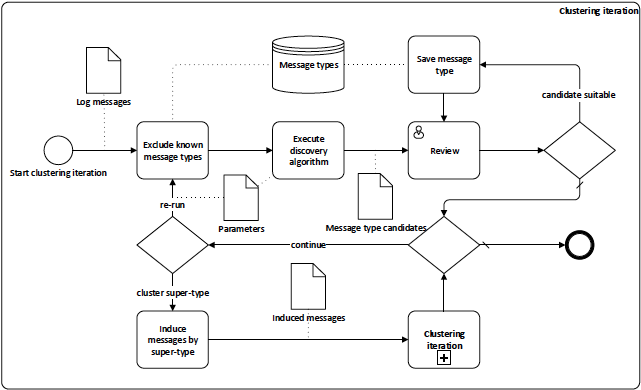
\includegraphics[width=\textwidth]{images/RURC.png} 	
 \end{minipage}
  \caption{Trvanie eng.py }
  \label{fig:eng-duration}
\end{figure}

\subsection{Mined patterns}
Rozhranie prezentuje stránkovací zoznam finalizovaných parsovacích vzorov, ktoré je možné si vyfiltrovať podľa zdrojovej aplikácie a jej verzie. Aktuálny vyfiltrovaný zoznam si užívateľ vie exportovať do formátu REtrie. Zoznam ďalej umožnuje náhľad na správy, ktoré boli vygenerované použitím vybraného parsovacieho vzoru. 

\begin{figure}[htbp]
 \centering 
 \begin{minipage}{0.95\linewidth}
 	\centering
 	\missingfigure[figheight=5cm]{Obrazok patternov}
 	%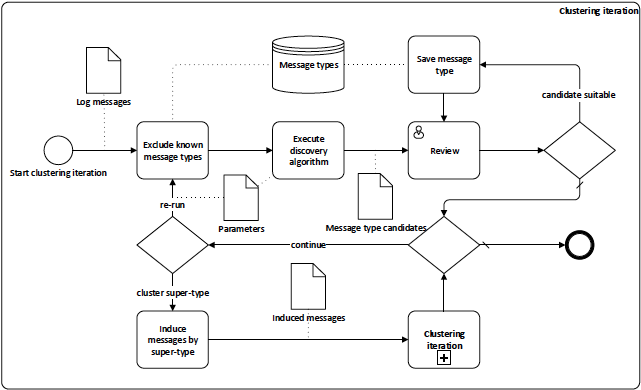
\includegraphics[width=\textwidth]{images/RURC.png} 	
 \end{minipage}
  \caption{Trvanie eng.py }
  \label{fig:eng-duration}
\end{figure}

\subsection{Regex Groups}
Zobrazuje zoznam sád typov regulárnych výrazov, ktoré sú v aplikácií nahrané. V systéme sme prednastavili základnú sadu, ktorá by mala byť postačujúca pre značnú časť prípadov a táto sada nejde zo systému zmazať. Systém ďalej umožnuje nahrať novú sadu zo súboru vo formáte :

 \begin{figure}[htbp]
 \centering 
 \begin{minipage}{0.95\linewidth}
 	\centering
 	\missingfigure[figheight=7cm]{Regex group}
 	%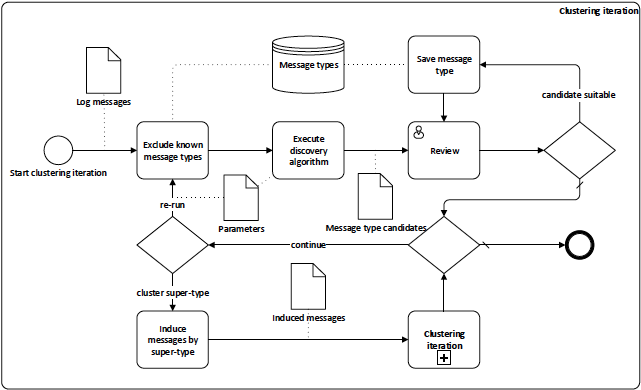
\includegraphics[width=\textwidth]{images/RURC.png} 	
 \end{minipage}
  \caption{Trvanie eng.py }
  \label{fig:eng-duration}
\end{figure}

\section{Inštalácia a nasadenie}
Implementovaná aplikácia používa len voľne dostupné knižnice a nástroje, ktoré sú schopné bežat na všetkých majoritných operačných systémoch. Predpokladáme ale, že aplikácia bude hlavne nasadená na linuxový server ako je to bežné. Preto sme vytvorili scripty, ktoré by mali administrátorovi pomôcť automatizovať proces nasadenia na linuxový server RHEL len za použitia nevyhnutne minimálnej konfigurácie. Použili sme pritom python virtuálne prostredie, konzolové nástroje Fabric a Ansible.

\subsection{Príprava prostredia}
V tejto fáze si aktivujeme python virtuálne prostredie a prostredníctvom pip balíčkovacieho manažéra si nainštalujeme Fabric.
Fabric je nástroj, ktorý nám dovolí písaním python kódu volať služby operačného systému. Týmto spôsobom: 

\begin{enumerate}
  \item Vygenerujeme ssh kľúče
  \item Prihlásime sa na cieľový systém a updatujeme ho
  \item Vytvoríme užívateľa a skupinu pod ktorou bude bežať naša aplikácia
  \item Nahrajeme vygenerované ssh kľúče
  \item Upgradujeme server a nainštalujeme závislosti pre Ansible
\end{enumerate}

\subsection{}